% Section content template for individual Educative lessons
% This file contains the actual content for a specific section
% Generated from Educative API section content

% Section: System Design: Twitter
% Section ID: 4687773419700224
% Section Slug: system-design-twitter
% Generated: 2025-12-08T12:05:47.655580

\subsection{Twitter}\label{RIdumTl9g4EDjqCEG1x22}
\\
Twitter is a free microblogging social network where registered users post messages called "Tweets". Users can also like, reply to, and retweet public tweets. Twitter has about 397 million users as of 2021, which is proliferating with time. One of the main reasons for its popularity is the vast sharing of breaking news on the platform. Another important reason is that Twitter allows us to engage with and learn from people belonging to different communities and cultures.\\
\strut \\

\begin{figure}[htbp]
 \centering
 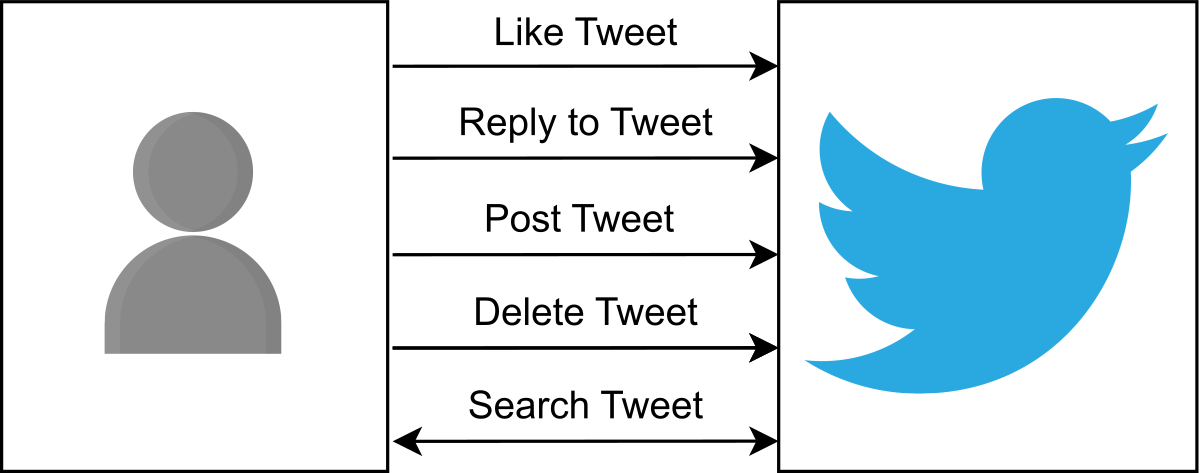
\includegraphics[width=0.25\textwidth]{Images/chapter_31/section_4687773419700224/5684743811366912.png}
 \caption{A user performs various operation on Twitter}
\end{figure}

The illustration below shows the country-wise userbase of Twitter as of January 2022 (source: Statista), where the US is taking the lead. Such statistics are important when we design our infrastructure because it allows us to allocate more capacity to the users of a specific region, and traffic served from near specific users.

\begin{figure}[htbp]
 \centering
 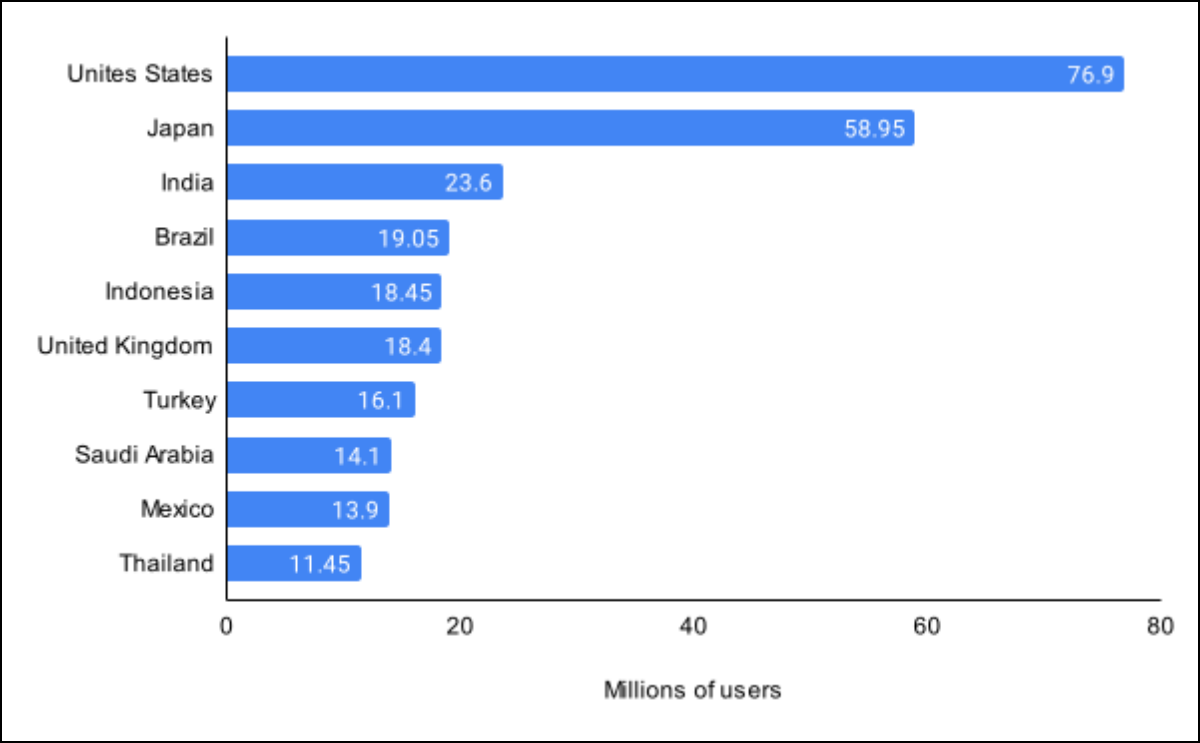
\includegraphics[width=0.5\textwidth]{Images/chapter_31/section_4687773419700224/6531721520742400.png}
 \caption{Country wise userbase on Twitter }
\end{figure}

\subsection{How will we design Twitter?}\label{S3Ew03tX1_5pZ9rHozjmB}
\\
We'll divide Twitter's design into four sections:

\begin{enumerate}
\item
\protect\phantomsection\label{prieBFGaOlDnsWVMuYu9l}
\href{https://www.educative.io/courses/grokking-the-system-design-interview/requirements-of-twitters-design}{\textbf{Requirements}}: This lesson describes the functional and non-functional requirements of Twitter. We'll also estimate multiple aspects of Twitter, such as storage, bandwidth, and computational resources.
\item
\protect\phantomsection\label{r5FECyjxOGOaH14IgrStM}
\href{https://www.educative.io/courses/grokking-the-system-design-interview/high-level-design-of-twitter}{\textbf{Design}}: We'll discuss the high-level design of Twitter in this lesson. We also briefly explain the API design and identify the significant components of the Twitter architecture. Moreover, we will discuss how to manage the Top-k problem, such as Tweets liked or viewed by millions of users on Twitter.
\item
\protect\phantomsection\label{5Nq27q1EREm1w-BnpNL5l}
\href{https://www.educative.io/courses/grokking-the-system-design-interview/client-side-load-balancer-for-twitter}{\textbf{Client-side load balancers}}: This lesson discusses how Twitter performs load balancing for its microservices system to manage billions of requests between various services' instances. Furthermore, we also see why Twitter uses a customized load-balancing technique instead of other commonly used approaches.
\item
\protect\phantomsection\label{2_i-DPA9w480iQgo-W6jN}
\href{https://www.educative.io/courses/grokking-the-system-design-interview/quiz-on-twitters-design}{\textbf{Quiz}}: Finally, we'll reinforce major concepts of Twitter design with a quiz.
\end{enumerate}
\\
Let's begin with defining Twitter's requirements.

% End of section content